% =================================================================================================
% File:			dp_strutturali.tex
% Description:	Defiinisce la sezione relativa a ...
% Created:		2015-03-26
% Author:		Tesser Paolo
% Email:		tesser.paolo@mashup-unipd.it
% =================================================================================================
% Modification History:
% Version		Modifier Date		Change											Author
% 0.0.1 		2015-03-26 			sistemato header								Tesser Paolo
% =================================================================================================
% 0.0.2			2015-04-08			aggiunto scheletro per pattern Facade			Tesser Paolo
% =================================================================================================
% 0.0.3			2015-04-14			descritto pattern Facade						Tesser Paolo
% =================================================================================================
% 0.0.4			2015-04-14			descritto pattern Adapter						Tesser Paolo
% =================================================================================================
%

% CONTENUTO DEL CAPITOLO

\subsection{Design pattern strutturali} % (fold)
\label{sub:design_pattern_strutturali}

	\subsubsection{Adapter (object)} % (fold)
	\label{ssub:adapter_object}
		\begin{itemize}
			\item \textbf{Scope dell'utilizzo}: questo pattern è utilizzato quando si vogliono utilizzare librerie esterne che però hanno interfacce diverse rispetto quelle utilizzate dall'applicazione. Per non modificare quindi parte del codice che utilizza queste componenti, le interfacce vengono adattate passando per una interna già esistente che farà da tramite con quella esterna;
			\item \textbf{Contesto dell'utilizzo}:
				\begin{itemize}
					\item \textbf{Client}: viene utilizzato nel package \texttt{client::model::services} per utilizzare un modulo \texttt{ng-auth} esterno che fornisce i servizi necessari per le operazioni di autenticazione, basato sui token, senza che vengano implementati dal gruppo.
					\begin{figure}[htbp]
						\centering
						\centerline{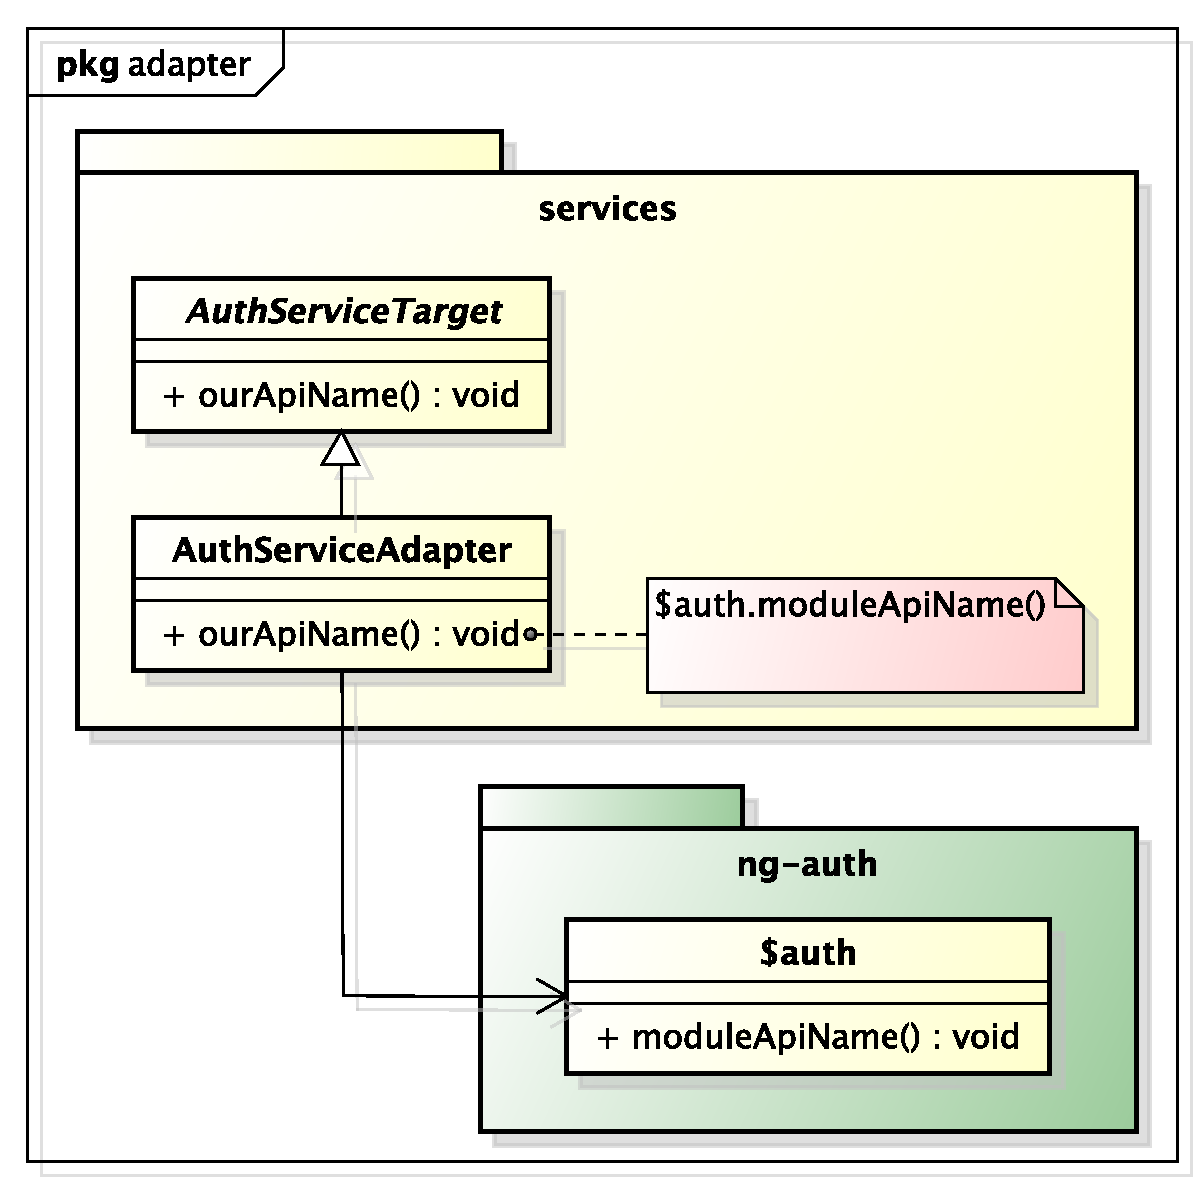
\includegraphics[scale=0.55]{./images/design_pattern_client/client_adapter.pdf}}
						\caption{Contestualizzazione Adapter - Client}
					\end{figure}
				\end{itemize}
		\end{itemize}
	% subsubsection adapter_object (end)

	\subsubsection{Fa\c{c}ade} % (fold)
	\label{ssub:facade}
		\begin{itemize}
			\item \textbf{Scope dell'utilizzo}: questo pattern è utilizzato per fornire un'interfaccia di alto livello unificata di tante interfacce di un sotto sistema più complesso. Questo rende più semplice al client interagire con quel sistema senza preoccuparsi di come le cose vengono implementate da esso;
			\item \textbf{Contesto dell'utilizzo}:
				\begin{itemize}
					\item \textbf{Client}: viene utilizzato direttamente da AngularJS in alcuni servizi come quello \$http o \$resource che permettono all'utilizzatore di non sapere come viene effettivamente implementata la chiamata alle API, effettuandola quindi in maniera più semplice di come è realmente. \newline
					Non ne viene fornita nessuna rappresentazione grafica in quanto non è una cosa che viene progettata dal team, ma usata direttamente attraverso il framework scelto.
				\end{itemize}
		\end{itemize}
	% subsubsection facade (end)


	\subsubsection{Front controller} % (fold)
	\label{ssub:front_controller}
		\begin{itemize}
			\item \textbf{Scope dell'utilizzo}: questo pattern è utilizzato per fornire un'unica entità con lo scopo gestire tutte le richieste in entrata da un determinato modulo dell'applicativo. Il Front Controller può inoltre effettuare semplici check o operazioni a seconda dei dati in entrata o lasciare l'elaborazione della richiesta ad una seconda entità, il Dispatcher, il quale si occupa di far confluire tale richiesta al relativo comando contenente la logica per soddisfarla. In questo modo, oltre a creare una gestione centralizzata delle richieste, si crea una divisione tra la logica di implementazione delle richieste e le modalità con cui quest'ultime vengono ricevute ed assegnate;
			\item \textbf{Contesto dell'utilizzo}:
				\begin{itemize}
					\item \textbf{Server}: tale pattern è utilizzato dalle classi appartenenti al package \texttt{server::processor} in cui il Front Controller è rappresentato dalla classe \texttt{RequestHandler} che si occupa di ricevere tutte le richieste del client, provenienti dalle classi del package	\texttt{server::endpoints}. La classe \newline \texttt{CommandDispatcher}, inoltre, si occupa di far confluire tali richieste al relativo comando. \newline
					[TO DO] (grafico del pattern applicato al caso di utilizzo nell'applicativo)
				\end{itemize}
		\end{itemize}
		% subsubsection front_controller (end)
% subsection design_pattern_strutturali (end)
